\chapter{用語まとめ}

\section{esa}

  \begin{figure}[H]
    \centering
    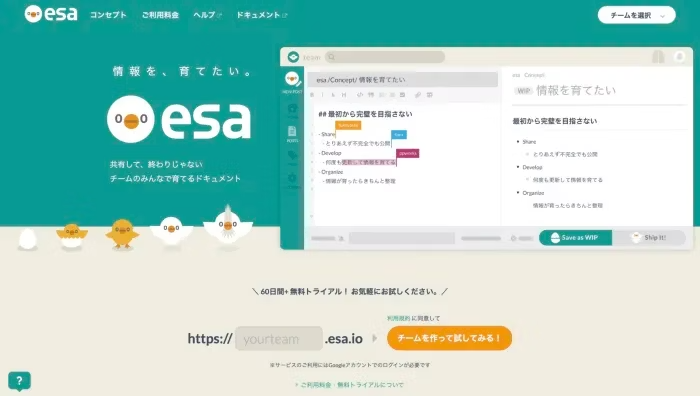
\includegraphics[width=6cm]{./image/02-chap3/esa.png}
    \caption{esaのホームページの写真}
    \label{chap3-esa-image}
  \end{figure}


  \begin{tcolorbox}[title=esaとは]
    esaとは、2014年に設立された合同会社esaの「情報共有ツール」です。
    esaは「不完全でも早い段階でチームに共有し、更新を重ねることでより良い情報に育つ」という発想のもと生まれました。そのため「Share(公開)」「Develop(更新して情報を育てる)」「Organize(育った情報を整理)」の3つの流れで設計されています。
    現在は3,000社を超える企業に導入されており、主に情報の蓄積やWIP機能(書いている途中でも共有する機能)を用いて、業務の効率化を実現している企業が多いです。
    \cite{esaとは} \cite{公式esaWeb}

  \end{tcolorbox}

\section{hugo}

  \begin{figure}[H]
    \centering
    
\includegraphics[width=6cm]{./image/02-chap3/hugo.png}
    \caption{hugoのホームページの写真}
    \label{chap3-hugo-image}
  \end{figure}

  \begin{tcolorbox}[title=hugoとは]
    HugoはGo言語で実装された「Webサイト構築フレームワーク」で、最初の公開は2013年という比較的新しいツールだ。コンテンツ管理システムではなく「Webサイト構築フレームワーク」と名乗っているとおり、コンテンツの管理ではなく、Webサイトで使われるHTMLファイルやRSSファイルなどの生成に特化した機能を備えている。
    \cite{hugoとは} \cite{hugo公式}
  \end{tcolorbox}

\section{GitHub Actions}

  \begin{figure}[H]
    \centering
    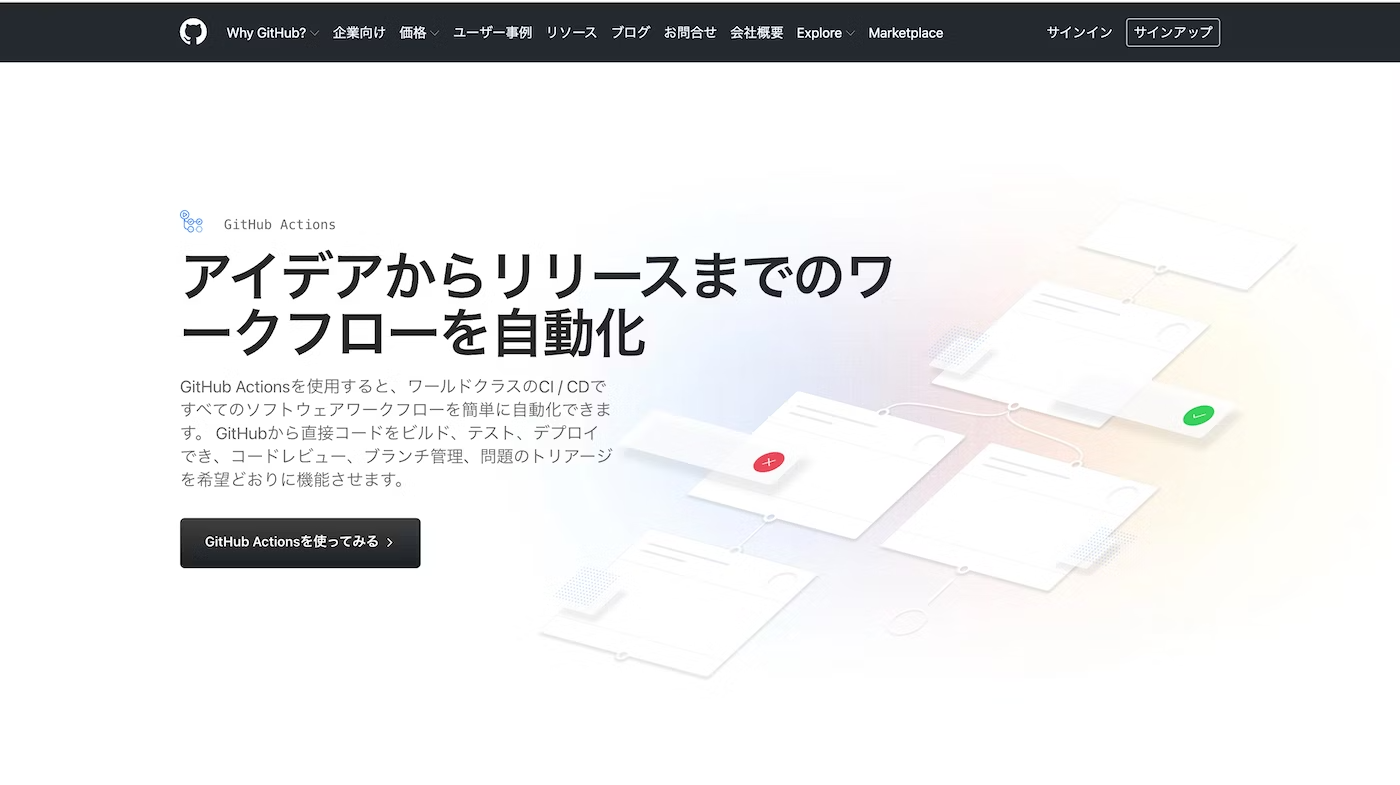
\includegraphics[width=6cm]{./image/02-chap3/githubActions.png}
    \caption{GitHub Actionsのホームページの写真}
    \label{chap3-githubAction-image}
  \end{figure}

  \begin{tcolorbox}[title=GitHub Pagesとは]
    GitHub Actionsで、ソフトウェア開発ワークフローをリポジトリの中で自動化し、カスタマイズし、実行しましょう。 CI/CDを含む好きなジョブを実行してくれるアクションを、見つけたり、作成したり、共有したり、完全にカスタマイズされたワークフロー中でアクションを組み合わせたりできます。
    \cite{githubAction}
  \end{tcolorbox}

\section{GitHub Pages}

  \begin{tcolorbox}[title=hugoとは]
    GitHub Pages は、GitHub のリポジトリから HTML、CSS、および JavaScript ファイル を直接取得し、任意でビルドプロセスを通じてファイルを実行し、ウェブサイトを公開できる静的なサイトホスティングサービスです。
    \cite{githubPages}
  \end{tcolorbox}


\section{CMS}

  \begin{tcolorbox}[title=CMSとは]
    「CMS」とは、「Contents Management System:コンテンツ・マネジメント・システム」の略で、簡単にいうとWebサイトのコンテンツを構成するテキストや画像、デザイン・レイアウト情報(テンプレート)などを一元的に保存・管理するシステムのことです。
    \cite{cmsとは}
  \end{tcolorbox}

